\documentclass[10pt]{article}
\usepackage{graphicx}
\usepackage{array}
\usepackage{xcolor}
\usepackage[a4paper,total={8in,10in}]{geometry}
\usepackage{mdframed}
\usepackage{geometry}
\usepackage{hyperref}
\renewcommand{\familydefault}{\sfdefault}
\usepackage[scaled=1]{helvet}
\usepackage[helvet]{sfmath}
\everymath={\sf}
\definecolor{capri}{rgb}{0.0, 0.75, 1.0}
\definecolor{caribbeangreen}{rgb}{0.0, 0.8, 0.6}
\definecolor{dartmouthgreen}{rgb}{0.05, 0.5, 0.06}
\definecolor{orange}{HTML}{FF7F00}
\definecolor{theme}{HTML}{273941}
\usepackage{multicol}

\begin{document}
\begin{mdframed}[backgroundcolor=theme]

\begin{minipage}{0.4\textwidth}
\begin{flushleft}
\vspace{1mm}

    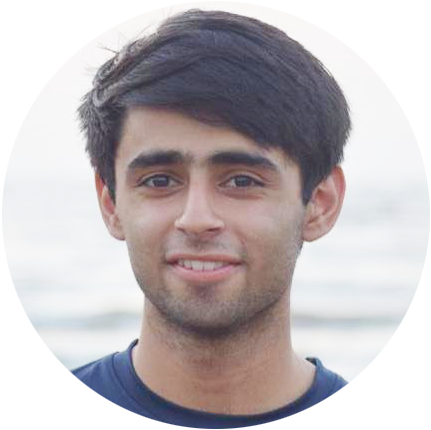
\includegraphics[scale=0.35]{picture.png}
\vspace{0.5mm}

\end{flushleft}

\end{minipage}
\begin{minipage}{\textwidth}
%\begin{mdframed}[backgroundcolor=black!80]


\begin{minipage}{0.55\textwidth}

\color{white}\textbf{\Huge{S H I V A M  \hspace{2mm}  G R O V E R}}\raggedright


\vspace{3mm}
\color{white}{\textit{\large{A Passionate and open-minded learner}}}
\vspace{5mm}

\end{minipage}




\end{minipage}
\end{mdframed}

\begin{minipage}{0.5\textwidth}

%\color{black!70}{\large{\textbf{Address: } Third floor, 8/21 West Patel Nagar}}\raggedleft
\vspace{5mm}
\hspace{3mm}
\begin{tabular}{l l}\raggedleft
\color{black!70}\textbf{Address}-& \color{black!70}3rd Floor, 8/21, West Patel Nagar, \\  
    
    & \color{black!70}New Delhi,110008\\

\end{tabular}
\end{minipage}
\begin{minipage}{0.4\textwidth}

%\color{black!70}{\large{\textbf{Address: } Third floor, 8/21 West Patel Nagar}}\raggedleft
\vspace{5mm}
\begin{flushright}
\begin{tabular}{l l}\raggedleft

\color{black!70}\textbf{Phone}-& \color{black!70}+91 9910998082\\ 
%textbf{Mother's Name}-& Mrs. Mitu Diddee\\
\color{black!70}\textbf{Email}-& \color{black!70}shivumgrover99@gmail.com\\
\color{black!70}\textbf{Github}-& \color{black!70}GitHub.com/shivumgrover\\
\color{black!70}\textbf{LinkedIn}-& \color{black!70}linkedin.com/in/shivam-grover-a61385167\\
\end{tabular}
\end{flushright}
\end{minipage}



\begin{center}
\line(1,0){560}
\end{center}

\begin{minipage}{0.95\textwidth}
\vspace{5mm}
\begin{huge}
\textbf{\color{theme}CAREER OBJECTIVES}
\end{huge}
\begin{mdframed}[backgroundcolor=theme]
\end{mdframed}

\vspace{1mm}

\color{black}\normalsize{{I am a motivated student, always trying to push my limits and explore my potential by trying new things out. I have a passion for solving real world problems using my code, while keeping the aesthetic part of the solution strong. I see myself in the near future working with a team, making products that help the world be a better place.
}}
\vspace{5mm}
\end{minipage}




\begin{minipage}{0.95\textwidth}
\vspace{5mm}
\begin{huge}
\textbf{\color{theme}EDUCATIONAL QUALIFICATIONS}
\end{huge}
\begin{mdframed}[backgroundcolor=theme]
\end{mdframed}

\vspace{1mm}

\begin{tabular}{||m{4cm}|m{4cm}|m{2cm}|m{3cm}||}
\hline
\hline

\begin{center}
\textbf{Course/Examination}
\end{center} & \begin{center}
\textbf{Institute/University}
\end{center} & \begin{center}
\textbf{Year of Passing}
\end{center} & \begin{center}
\textbf{Performance}
\end{center}\\
\hline
&&&\\
\begin{center}
B.Tech in Information Technology
\end{center} & \begin{center}
Bharati Vidyapeeth's College of Engineering, New Delhi
\end{center} & \begin{center}
2021
\end{center} & \begin{center}
CGPA 7.59
\end{center}\\
\hline
\begin{center}
AISSCE(Science with PCM) XII CBSE
\end{center} & \begin{center}
Bharati Vidya Bhavan's, Mehta Vidyalaya, New Delhi
\end{center} & \begin{center}
2017
\end{center} & \begin{center}
88.4%
\end{center}\\
\hline
\begin{center}
AISSE X CBSE
\end{center} & \begin{center}
Bharati Vidya Bhavan's, Mehta Vidyalaya, New Delhi
\end{center} & \begin{center}
2015
\end{center} & \begin{center}
CGPA 8.8
\end{center}\\
\hline
\hline

\end{tabular}

\end{minipage}


\begin{minipage}{0.95\textwidth}
\vspace{5mm}
\begin{huge}
\textbf{\color{theme}PROJECTS}
\end{huge}
\begin{mdframed}[backgroundcolor=theme]
\end{mdframed}

\vspace{1mm}

\color{black}\normalsize{{
\begin{enumerate}
\item\color{black} An application for e-Charging Station Operators to maximise their earnings and attract more customers using dynamic pricing solutions (Winning project in Smart India Hackathon 2019)\\
	\color{capri}\url{https://github.com/shivumgrover/EazyCharge}
\color{black} \item  Autonomous Black Line Following robot for picking up and dropping of metallic objects using an electromagnet and a mechanical arm (Winning project in e-Yantra 2019, theme Thirsty Crow)\\
 	\color{capri}\url{ https://github.com/shivumgrover/Eyantra-Thirsty_Crow-Team_ID-972}

\color{black} \item  Android Application for easy boarding of buses, especially for the disabled, elderly and children(Winning project in HackBVP 2.0)\\
	\color{capri}\url{https://github.com/shivumgrover/BoardEasy}
	
 \color{black} \item  Autonomous Life Boat(finalist in Arduino Day Hackathon @ BVP 2019)\\
	\color{capri}\url{https://github.com/shivumgrover/Autonomous-Life-Boat}
 \color{black} \item  Android Application for women safety using Geolocation (Runners up in IGDTU hackathon 2018)
	\color{capri}\url{https://github.com/shivumgrover/Aarogya_Women_Safety}
	
\color{black} \item  Android application for home automation using Raspberry Pi\\
	\color{capri}\url{https://github.com/shivumgrover/ISTY-home-automation}

\color{black} \item  Android application for Waste segregation using Firebase ML Kit (Winning project at NIEC hackathon 2018)
\color{black} \item  A health assistant based android application which provides you with a personalized diet plan taking into consideration several factors such as your Body fat percentage(calculated using computer vision),your current heart rate(calculated using camera flash), your nutrient deficiencies etc. Other features included posture correction for exercises and aerobics by Augmented reality\\
	\color{capri}\url{https://github.com/shivumgrover/SwasthyaIGNITE}

\color{black} \item Android Application for facilitating seamless traversal of emergency vehicles using Google Maps and Machine Learning\\




\end{enumerate}
}}
\vspace{2mm}
\end{minipage}



\end{document}
